% ALL PARTS OF THIS DOCUMENT HAVE BEEN MOVED TO WFS_DOC.TEX AND RELATED FILES.  PLEASE CONTINUE ALL WORK THERE. June 11, 2014. 

\documentclass{article}

\usepackage[utf8]{inputenc}
\usepackage[english]{babel}
\usepackage{mathrsfs,amsmath}
\usepackage{float}
\usepackage{subfig}
\usepackage{graphicx}

% Puts captions of tables on top
\floatstyle{plaintop}
\restylefloat{table}

% Puts captions in bold
\captionsetup{labelfont=bf}

\begin{document}
\section{The Fraunhofer Approximation}
The Fraunhofer approximation is a more stringent approximation of the Fresnel approximation which is valid when
\begin{equation}
z\gg\frac{2\pi(\xi^2+\eta^2)_{\text{max}}}{2\lambda},
\label{eq:strong_con}
\end{equation}
where $\lambda$ is the wavelength and ($\xi,\eta$) are the 2 dimensional positions on the aperture plane. It is used to compute wave propagation in the far field, whereas the Fresnel approximation is used to compute wave propagation in the near field. Another condition for the Fraunhofer approximation, which as well applies to the Fresnel approximation, is that the incident waves must be within the paraxial regime, meaning that the direction of propagation must be small towards the optical axis of the system. In other words, this is simply a restriction to small incident angels. A less stringent condition to Equation \eqref{eq:strong_con} is 
\begin{equation}
z>\frac{2D^2}{\lambda},
\label{eq:normal_con}
\end{equation}
where $D$ is the dimension of the aperture. Although the distance $z$ requires to be large, the Fraunhofer diffraction patterns can still be observed at distances much closer than implied by the above conditions. 

The observed field strength $U(x,y)$ can be calculated by the Fraunhofer approximation as
\begin{equation}
U(x,y)=\frac{e^{jkz}e^{j\frac{k}{2z}(x^2+y^2)}}{j\lambda z}\iint\limits_{-\infty}^{~~~\infty} \left. U(\xi,\eta)e^{-j2\pi(f_X\xi+f_Y\eta)}d\xi d\eta \right|_{f_X=\frac{x}{\lambda z},f_Y=\frac{y}{\lambda z}},
\label{eq:fraunhofer}
\end{equation}
with $k=2\pi/\lambda$ the wavenumber and where $U(\xi,\eta)$ is the field distribution at the aperture. From this equation it can be seen that the Fraunhofer approximation simply is the Fourier Transform (FT) of the distribution $U(\xi,\eta)$ times a multiplicative factor, evaluated at frequencies $f_X$ and $f_Y$.

\section{Diffraction Patterns at the Focal Plane of a Single Lens}
Here we assume a diffraction-limited system with the input directly placed against the lens, to model the lens system for our purposes that is used to measure the intensity in the focal plane. The input $U_i(\xi,\eta)$ then contains the disturbance induced by the atmosphere and is illuminated by the solar system which has a flat wavefront. The field distribution behind the lens is then calculated by
\begin{equation}
U^\prime_i(\xi,\eta)=U_i(\xi,\eta)P(\xi,\eta)e^{-j\frac{k}{2f}(\xi^2 + \eta^2)},
\label{eq:dis_behind_lens}
\end{equation}
where $P(\xi,\eta)$ is the pupil function of the lens system and is defined by
\begin{equation}
P(\xi,\eta)= \begin{cases} 1 & \text{inside the aperture} \\ 0 & \text{otherwise.} \end{cases}
\end{equation}
Moreover the exponential function in Equation \eqref{eq:dis_behind_lens}, is the phase change introduced by the lens with focal length $f$. Using the Fresnel diffraction formula the field distribution in the back focal plane of the lens can be found as
\begin{equation}
U_f(x,y)=\frac{e^{jkf}e^{j\frac{k}{2f}(x^2+y^2)}}{j\lambda f}\iint\limits_{-\infty}^{~~~\infty} \left. U_i(\xi,\eta)P(\xi,\eta)e^{-j2\pi(f_X\xi+f_Y\eta)}d\xi d\eta \right|_{f_X=\frac{x}{\lambda z},f_Y=\frac{y}{\lambda z}}.
\label{eq:fresnel}
\end{equation}
Hence the complex amplitude field distribution in the back focal plane of the lens is simply the Fraunhofer diffraction pattern seen in Equation \eqref{eq:fraunhofer}, but with the propagation distance $f$ instead of $z$. Thus the Fraunhofer diffraction patterns can be observed although not satisfying the before discussed conditions \eqref{eq:strong_con} and \eqref{eq:normal_con}. The real interest is the intensity across the focal plane and is computed by
\begin{equation}
I_f(x,y)=|U_f(x,y)|^2.
\end{equation}
Also the model of the lens system as derived here is studied under the condition that the illumination is monochromatic. 


The above text is based on (\textbf{Goodman,2005}) and is also advised for further reading.

\section{Numerical Computation of the Intensity Distribution in the Focal Plane for a Single Lens}
The computation of the FT will be done numerically. This can be done in a highly efficient algorithm called the Fast Fourier Transform (FFT). Using the Discrete Fourier Transform (DFT) it approximates the continuous FT of a function $g(x)$, where the FT of a two dimensional function is defined as
\begin{equation}
\hat{g}(f_X,f_Y)=\iint\limits_{-\infty}^{~~~\infty} g(x,y)e^{-j2\pi(f_Xx + f_Yy)}dxdy.
\end{equation}
A first approximation is restricting the integral to the finite interval $-L_x/2 \leq x \leq L_y/2$ and $-L_y/2 \leq y \leq L_y/2$, giving us, for $L=L_x=L_y$,
\begin{equation}
\hat{g}(f_X,f_Y)\approx\iint\limits_{-L/2}^{~~~L/2} g(x,y)e^{-j2\pi(f_Xx + f_Yy)}dxdy.
\end{equation}
Where the size $L_x$ and $L_y$ must be large enough to cover the essential non-zero parts of the function $g(x,y)$. Second the integral is approximated by replacing it by a finite sum, then we get
\begin{equation}
\hat{g}(f_X,f_Y)\approx  \Delta y \sum\limits_{m=N_y/2}^{N_y/2} e^{-j2\pi mf_Y\Delta y}\Delta x\sum\limits_{n=-N_x/2}^{N_x/2}g(n\Delta x,m\Delta y)e^{-j2\pi nf_X\Delta x },
\end{equation}
where the $x,y$-coordinates are sampled in the before described intervals with $N_x,N_y$ samples, when $N=N_x=N_y$, spaced at $\Delta x=\Delta y = L/N$ at positions $x_n=n\Delta x$ and $y_m=m\Delta y$ with $n=m=-N/2,...,N/2-1$. A connection to the DFT can be made by sampling the spatial frequencies with $N$ values in the interval $-\Delta x/2 \leq f_X \leq \Delta x/2$ and $-\Delta y/2 \leq f_Y \leq \Delta y/2$, the samples being spaced by $\Delta f_X=\Delta f_Y=1/L$ at frequencies $f_k=k\Delta f_X$ and $f_l=l\Delta f_Y$, with $k=l=-N/2,...,N/2-1$. This produces the exact DFT described by
\begin{equation}
\hat{g}(k\Delta f_X,l\Delta f_Y)\approx  \Delta y \sum\limits_{m=N_y/2}^{N_y/2} e^{-j2\pi lm/N_y}\Delta x\sum\limits_{n=-N_x/2}^{N_x/2}g(n\Delta x,m\Delta y)e^{-j2\pi kn/N_x}.
\end{equation}
In short the procedure is:
\begin{enumerate}
	\item sampling the function $g(x,y)$ in a grid at values $(x_n,y_m)$ and storing the values in a matrix of size $(N_x,N_y)$,
	\item doing a DFT on this matrix and multiplying it with the sample spacings $\Delta x$ and $\Delta y$,
	\item plotting the resulting matrix of size $(N_x,N_y)$ at points $(f_k,f_l)$ in the spatial frequency space.
\end{enumerate}

The numerical calculation of the diffraction pattern is now easily done by applying the FFT to $U_i(\xi,\eta)P(\xi,\eta)$ adding the multiplicative factor as seen in Equation \eqref{eq:fresnel} and setting $(f_k=\frac{x_k}{\lambda z},f_l=\frac{y_l}{\lambda z})$. The intensity distribution is then found by taking the modulus squared.

\section{The Intensity Distribution of a Lenslet Array}
Every intensity distribution of a lenslet is calculated separately by the procedure discussed above.
If the incident rays enter on a to big angle, the FFT will be incorrect. To solve this, the average tilt of the incident phase on a lenslet is calculated. From this tilt a shift of the intensity distribution can be calculated. Putting this into a loop we calculate every intensity distribution of every lenslet with the correct coordinates. Then the distributions are interpolated on a grid that represent the Charge-Couple Device (CCD) giving the complete intensity distribution. 

\section{Answers to assignment questions} 
\begin{enumerate}
\item 
	In figure \ref{fig:num_vs_an} the difference is seen between the numerical solved diffraction pattern and the analytically solved diffraction pattern. Clearly the two are almost identically except for the outer rings where the flaws of numerical computation are seen through the not disk like shape in the airy function. Because only the first few orders of the airy disk are important this is a good approximation to be used for calculating the centroids. 
	\begin{figure}[H]
		\centering
			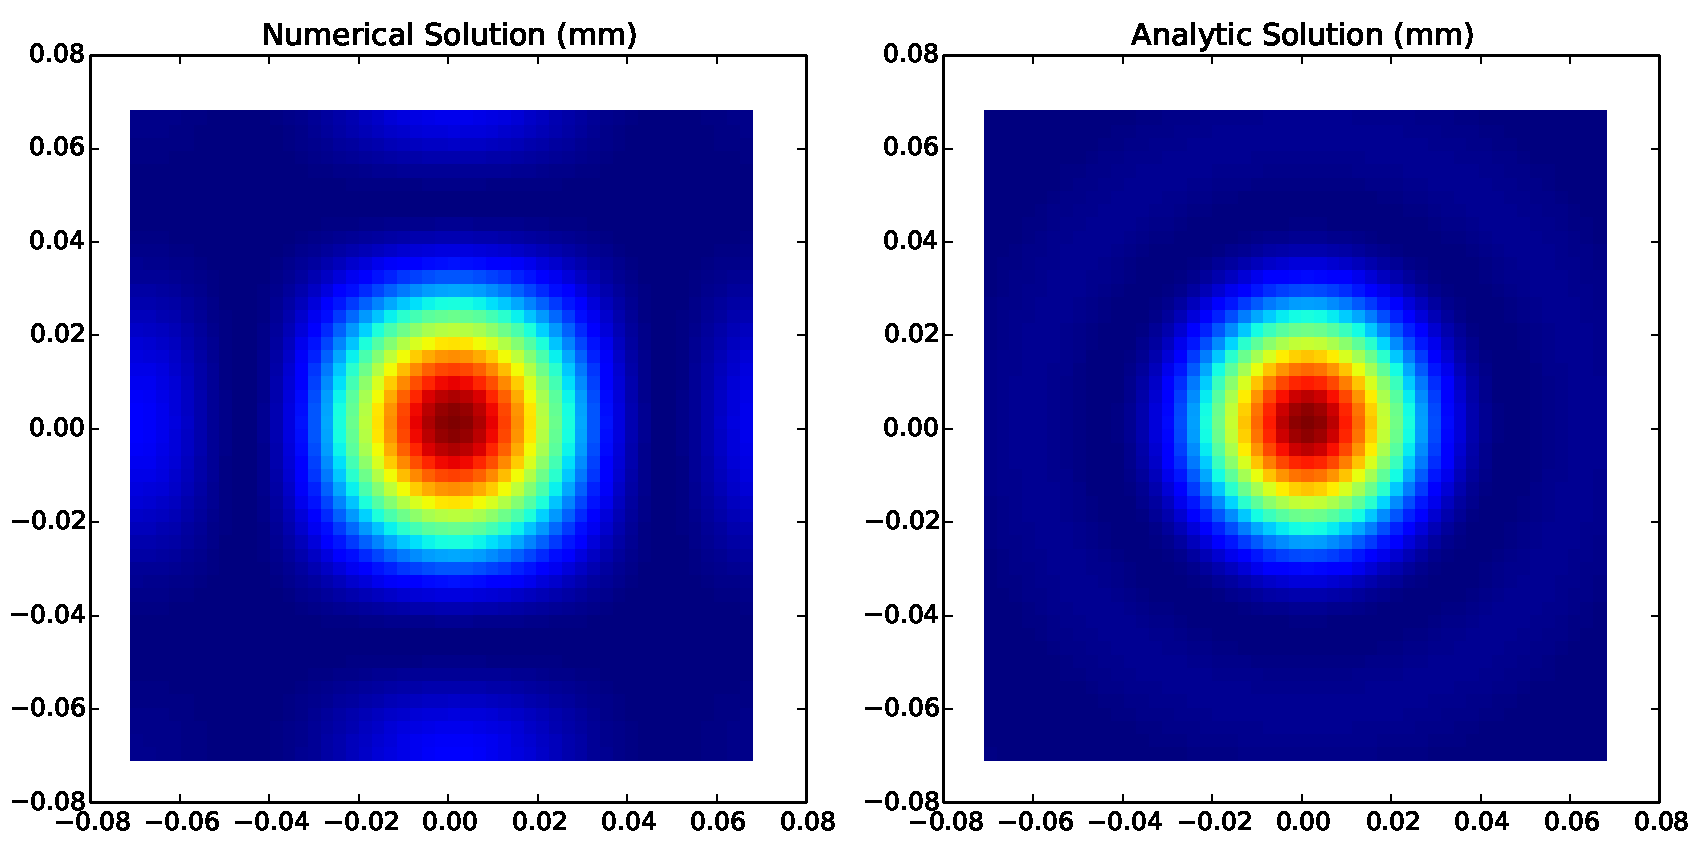
\includegraphics[width=1.0\textwidth]{./figures/num_vs_an.pdf}
		\caption{Numerical solution VS analytical solution}
		\label{fig:num_vs_an}
	\end{figure}
\item

\end{enumerate}

\end{document}